Knowledge bases organize and store factual knowledge, enabling
a multitude of applications including question answering~\cite{yao2014information,bao2014knowledge,seyler2015generating,hixon2015learning,bordes2015large,dong2015question} and information retrieval~\cite{kotov2012tapping,dalton2014entity,xiong2015query,xiong2015esdrank}.
Even the largest knowledge
bases (e.g. DBPedia, Wikidata or Yago), despite enormous effort invested in their maintenance, are incomplete, and the lack of coverage
harms downstream applications. Predicting missing
information in knowledge bases is the main focus of statistical relational learning (SRL).

Following previous work on SRL, we assume that knowledge bases store collections of triples of the form (subject, predicate, object). Consider, for example, the triple (\textit{Mikhail Baryshnikov}, \textit{educated\_at}, \textit{Vaganova Academy}), where we will refer to {\it Baryshnikov} and {\it Vaganova Academy} as entities and to {\it educated\_at} as a relation. Additionally, we assume that entities are labeled with types (e.g.,  {\it Vaganova Academy} is marked as a {\it university}).
It is convenient to represent knowledge bases as directed labeled multigraphs with entities corresponding to nodes and triples encoded by labeled edges (see Figure~\ref{fig:kb}).

\begin{figure}[t!]
    \centering
    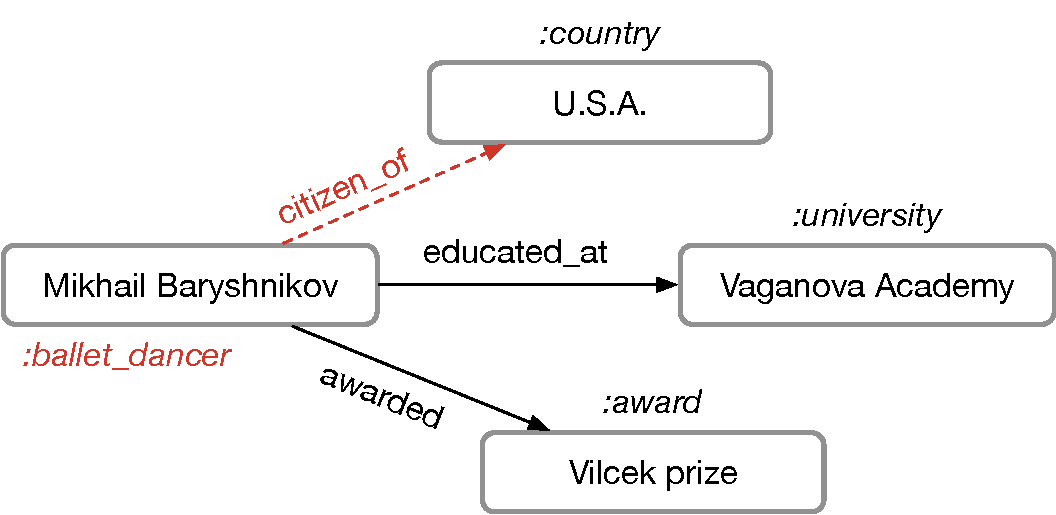
\includegraphics[width=0.95\linewidth]{figures/kb-example.pdf}
    \caption{A knowledge base fragment: The nodes are entities, the edges are relations labeled with their types, the nodes are labeled with entity types (e.g., {\it university}). The edge and the node label shown in red are the missing information to be inferred.}
    \label{fig:kb}
\end{figure}

We consider two fundamental SRL tasks: link prediction (recovery of missing triples) and entity classification (assigning types or categorical properties to entities). In both cases, many missing pieces of information can be expected to reside within the graph encoded through the neighborhood structure -- i.e.  knowing that \textit{Mikhail Baryshnikov} was educated at the \textit{Vaganova Academy} implies both that \textit{Mikhail Baryshnikov} should have the label person, and that the triple (\textit{Mikhail Baryshnikov}, \textit{lived\_in}, \textit{Russia}) must belong to the knowledge graph. Following this intuition, we develop an encoder model for entities in the relational graph and apply it to both tasks.

Our entity classification model, similarly to \citet{kipf2016semi}, uses softmax classifiers at each node in the graph. The classifiers take node representations supplied by a relational graph convolutional network (R-GCN) and predict the labels. The model, including R-GCN parameters, is learned by optimizing the cross-entropy loss.

Our link prediction model can be regarded as an autoencoder consisting of (1) an encoder: an R-GCN producing latent feature representations of entities, and (2) a decoder: a tensor factorization model exploiting these representations to predict labeled edges. Though in principle the decoder can rely on any type of factorization (or generally any scoring function), we use one of the simplest and most effective factorization methods: DistMult~\cite{distmult-embedding_entities_and_relations}. We observe that our method achieves competitive results on standard benchmarks, outperforming, among other baselines, direct optimization of the factorization (i.e.~vanilla DistMult).  This improvement is especially large when we consider the more challenging FB15k-237 dataset~\cite{toutanova2015observed}. This result demonstrates that explicit modeling of neighborhoods in R-GCNs is beneficial for recovering missing facts in knowledge bases.

Our main contributions are as follows. To the best of our knowledge, we are the first to show that the GCN framework can be applied to modeling relational data, specifically to link prediction and entity classification tasks. Secondly, we introduce techniques for parameter sharing and to enforce sparsity constraints, and use them to apply R-GCNs to multigraphs with large numbers of relations. Lastly, we show that the performance of factorization models, at the example of DistMult, can be significantly improved by enriching them with an encoder model that performs multiple steps of information propagation in the relational graph.
